

\frame
{
	\frametitle{Problem Formulation}
	
	\begin{itemize}[]
		\item<1->Given a set of $k$ real-time streams of events $S = \{ s_1,s_2, ..., s_k\}$.
		
		\item<1 -> Each stream $s_i=\langle e_1,e_3...,e_t,...\rangle$  is an evolving time-ordered sequence of events.
		
		\item<1 -> Each event is defined as a tuple of attributes $e_t = (type,\tau,id,a_1,a_2.....,a_n)$ where $type\ \in  \Sigma$ (i.e., event types). 
		\item<1-> A user-defined pattern (i.e., complex event of interest) $P$ expressed as sequence of event types.
		
		%  \item<1->Goal:  provides online prediction about when the event pattern $P$ is expected to be completed each single stream $s_i$ 
		
		\item<1->Goal: the main objective is to predict the pattern $P$ completion with certain probability in the future over each stream $s_i$ given the current time event $e_t$. 
	\end{itemize}
}

\begin{frame}[fragile]

	\frametitle{Illustrative Application:}
    \framesubtitle{Maritime Surveillance}
	\begin{itemize}
%		\item<only@1> Process  emitted from moving vessels or derived critical points of vessel trajectories as input event streams.
		\item<only@1> Event tuple (i.e., critical points) derived from raw Automatic Identification System (AIS) messages of moving vessels e.g., 
		\begin{minted}{json}
	{
	"timestamp":1443651492000,
	"id":"228133000",
	"annotation":"change_in_heading",
	"latitude":48.117775,
	"longitude":-4.4205885,
	"distance":323.406,
	"heading":264.27
	"speed":18.48,
	}
	\end{minted}
	
		\item<only@1> Example patterns such as 
		$P_1=\mathit{change\_heading} \cdot \mathit{gap\_start} \cdot \mathit{gap\_end} \cdot 
		\mathit{change\_heading}$ or $P_2=\mathit{Sailing}$
	\end{itemize}
\end{frame}


\frame
{
	\frametitle{Event Patterns Prediction System \footnote{ The source code can be\\ found here: \url{https://goo.gl/roj1ax}.}}
	%\framesubtitle{Maritime Surveillance}
	\begin{center}
		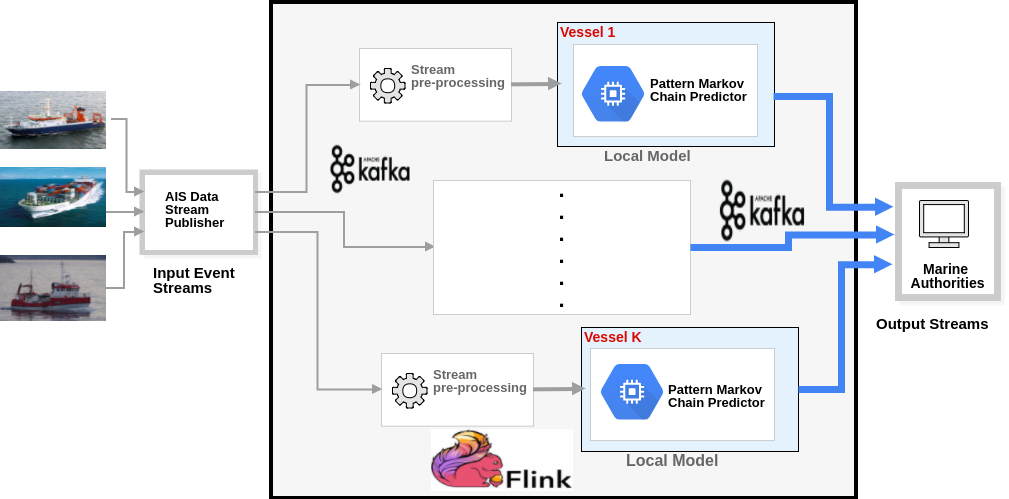
\includegraphics[width=1.05\textwidth,left]{figures/architecture.png}	\linebreak\\
	 System architecture and implementation for Maritime Surveillance.
		
%		emphasis on implementation // may add a slide // code link 
	\end{center}
}


\frame
{
	\frametitle{Event Patterns Prediction System}
	%\framesubtitle{Application Domain: Maritime Surveillance}
	\begin{itemize}
		
		\item<only@1> The system maintains a Pattern Markov Chain predictor for each vessel's stream. 
		\item<only@1> Developed in the context of the datAcron project \footnote{http://www.datacron-project.eu/}.
		\item<only@1> For large-scale processing support, the system was implemented based on the Apache Flink \citep{carbone2015apache} stream processing framework. 
	\end{itemize}
}